\documentclass{ieeeaccess}
\usepackage{cite}
\usepackage{amsmath,amssymb,amsfonts}
\usepackage{algorithm}
\usepackage{algorithmicx}
\usepackage{algpseudocode}
%% \usepackage{caption}
\usepackage{graphicx}
\usepackage{textcomp}

\usepackage{multirow}

\usepackage{array}
\setlength\extrarowheight{3pt}

\providecommand{\e}[1]{\ensuremath{\times 10^{#1}}}

\def\BibTeX{{\rm B\kern-.05em{\sc i\kern-.025em b}\kern-.08em
    T\kern-.1667em\lower.7ex\hbox{E}\kern-.125emX}}
\begin{document}
\history{Date of publication xxxx 00, 0000, date of current version xxxx 00, 0000.}
\doi{10.1109/ACCESS.2017.DOI}

\title{Using Fuzzy Systems as Agents' Rules in Multi-Agent Systems
for the Creation of Forex Market Predictive Models}

% \title{Using Intuitionistic Fuzzy Inference Systems For the Creation
% of an Agent-based Financial Market Model}
\author{
    \uppercase{Amaury Hernandez-Águila\authorrefmark{1},
    \uppercase{Mario García-Valdez\authorrefmark{1}
      and
    Juan-Julián Merelo-Guervós\authorrefmark{2}}}}
\address[1]{National Technological Institute of Mexico, Calzada Del Tecnológico s/n, Fraccionamiento Tomas Aquino, Tijuana, BC 22414 Mexico (e-mail: {amerhag,mario}@tectijuana.edu.mx)}
\address[2]{University of Granada, Campus Aynadamar Daniel Saucedo Aranda s/n, Granada 18071, 80523 Spain (e-mail: jmerelo@geneura.ugr.es)}
%% TODO 1: Grant information.
\tfootnote{This paragraph of the first footnote will contain support 
information, including sponsor and financial support acknowledgment. For 
example, ``This work was supported in part by the U.S. Department of 
Commerce under Grant BS123456.''}

%% TODO 2: Do we need to change this?
\markboth
{Author \headeretal: Preparation of Papers for IEEE TRANSACTIONS and JOURNALS}
{Author \headeretal: Preparation of Papers for IEEE TRANSACTIONS and JOURNALS}

\corresp{Corresponding author: Mario García-Valdez (e-mail: mario@tectijuana.edu.mx).}

% You must justify why do we care, in the beginning, 
% Why is this problem important?
% Why is this solution needed?
% Why is it better?
% Amaury: I state that the method is competitive. I don't want to
% Amaury: say that it is better because it is interpretable or anything
% Amaury: like that, because I didn't perform experiments to prove that.
% All this is very brief just a short sentence for each - Mario
% We will try not to use a Passive voice when we can - Mario
% TODO 3: COMPLETE.

\begin{abstract}
Financial market predictive models are tools that help us to understand a
market's behavior. Better and different methods for generating these
predictive models are needed in order to obtain different insights
about a market. This paper presents a method for creating forex market predictive models 
using multi-agent systems and fuzzy systems. Agents in the                 
multi-agent system represent traders that are issuing buy and sell
orders in a market. We use fuzzy systems to model the rules followed by
traders when they perform trades that would simulate the real
prices of a market. Activation functions are used to restrict the
agents' behavior to simulate the hesitancy of a trader to  
% Talk a bit about the type of activation functions 
% I think this is an important aspect of the paper - Mario
% TODO 4: COMPLETE.
perform a trade. Activation functions use the grades of membership
obtained from an agent's fuzzy system, along with thresholds obtained
from training data sets, to determine if that agent is specialized
enough to handle a market's current conditions. %
We performed experiments to demonstrate how capable our method is for
predicting future market prices.
Results demonstrate that our method is
competitive compared to predictive models generated using deep
learning, as well as models generated by random forest, AdaBoost,
XGBoost, and support-vector machines. Furthermore, experiments where
we compare our multi-agent systems with and without activation
functions show
% What kind of experiments? against who?
% TODO 5: COMPLETE.
that the use of activation functions to restrict the agents' behavior
help to obtain better predictive models.
\end{abstract}

\begin{keywords}
% TODO 6: COMPLETE. I added some of the keywords from Munkhdalai2019.
% I'm already using kewords from
% http://www.ieee.org/organizations/pubs/ani_prod/keywrd98.txt
  Economic forecasting, fuzzy systems, multi-agent system, activation function, forex market.
\end{keywords}

\titlepgskip=-15pt

\maketitle

\section{Introduction}
\label{section:introduction}

The prices of a financial market can be forecasted using different
techniques, such as the analysis of raw price data or news involving
the financial markets of interest \cite{Liu2019}. These approaches have
% These approaches ?
% Amaury: Yeah. Corrected.
the disadvantage of generating predictions for a market which are
entirely dependant on the trader's skills and knowledge about the
market being predicted. A more robust approach when handling raw price
data is the use of technical indicators \cite{Alsubaie2019}, which
preprocess a market's raw data to distill different aspects of it,
such as a market's volatility or general direction. In the case of
using news to draw predictions for a market, a more robust approach
would be the use of sentiment analysis \cite{LienMinh2018}
\cite{Cabrera2018}, which can draw conclusions about the general
sentiment about a financial market in order to know if prices will go
down or up. An important drawback of these methods is that we 
% Just removed the "approach" word to not sound repetitive (was used a few
% lines above) - M
% Amaury: Okie dokie.
are not obtaining explanations about why certain behavior occurred; we
are not generating a model about a market, we are simply distilling
the data. Predictive models can be created using a variety of
techniques, such as ARIMA \cite{Idrees2019} or hidden Markov models
\cite{Cao2019}, or machine learning techniques such as support-vector
machines (SVM) \cite{Guo2018} and neural networks \cite{Chen2019a}. A
drawback of some of these methods is that they generate \textit{black
box} models, i.e. it is difficult for a user to understand how the
model is processing its inputs. A technique that alleviates this
problem is fuzzy logic, which can also be used to create predictive
models \cite{Jiang2018} \cite{Sang2019} \cite{Chourmouziadis2019}.

% Talk about the drawbacks of these black box approaches - M
% Even if this is mentioned later, here is a good place - M
% TODO 7: COMPLETE.

% However, the work presented in this paper focuses on   
% forecasting the prices of financial markets, and we selected a set of
% machine learning techniques to create predictive models.
% This is not good, is weak. Why ? is it just a selection? 
% Explain why. Put here a list of why yours is a better solution:
% 1. It can be interprteted, 2. Is knowledge-based, 3. Is a simulation and not data-based ?, etc.
% You must first identify weak points in the methods above so we can see
% the benfits of our approach - M
% Amaury: I'm removing this part and justifying the method in the
% following paragraph.

The method presented in this paper uses a hybridization of fuzzy logic
and multi-agent systems (MAS). The use of fuzzy logic enables
the method to present results to the user that are easily
interpretable, especially if we use Mamdani fuzzy sets \cite{Mamdani1975} 
to create the membership functions of a fuzzy system, as in the
work of Abdulgader and Kaur \cite{Abdulgader2019}. %
% In contrast the approaches mentioned earlier do not provide ..
% TODO 8: COMPLETE. I just removed this incomplete sentence. I'm
% already explaining the drawback of black box models in the previous paragraph.
% I'm connecting this paragraph to the next one too.
In particular, we
propose the use of intuitionistic fuzzy logic (IFL)
\cite{Atanassov1986} \cite{Atanassov2003}, as IFL adds another layer
of interpretability for the fuzzy systems through the concept of
indeterminacy. Although there are alternatives to IFL, such as type-2
fuzzy systems, the defuzzification of IFL systems can be faster than
the aforementioned systems \cite{Hernandez-Aguila2016}, while also
providing comparable interpretability.

The work presented in this paper focuses on fuzzy logic and its
implementation through fuzzy systems. The use of fuzzy logic enables
the method to present results to the user that are easily
interpretable, especially if we use Mamdani fuzzy sets \cite{Mamdani1975} 
to create the membership functions of a fuzzy system, as in the
work of Abdulgader and Kaur \cite{Abdulgader2019}. In particular, we
propose the use of IFL
\cite{Atanassov1986} \cite{Atanassov2003}, as IFL adds another layer
of interpretability for the fuzzy systems through the concept of
indeterminacy. Although there are alternatives to IFL, such as type-2
fuzzy systems, the defuzzification of IFL systems can be faster than
the aforementioned systems \cite{Hernandez-Aguila2016}, while also
providing comparable interpretability. To our knowledge, IFL has not been
used for representing knowledge in financial predictive models. We
believe that IFL could be used to model a trader's uncertainty and
hesitancy when performing trades, and thus help us to better understand
the behavior of a market.
% Say something like.. to our knowledge IFL 
% has not been applied for representing knowledge for ... - M 
% We must do this in all applicable places. - M
% TODO 9: COMPLETE.
Fuzzy logic has proved to be useful in many fields, and one can find
many works involving financial market prediction using fuzzy systems,
such as the works by Tsai et al. \cite{Tsai2019} and Zeng et
al. \cite{Zeng2019}, where fuzzy time-series are used to perform the
predictions; as in the works by Rajab and Sharma \cite{Rajab2019} and
Vlasenko et al. \cite{Vlasenko2019}, where a neuro-fuzzy approach is
taken; or as in the works by Yue et al. \cite{Yue2019},
Witayakiattilerd \cite{Witayakiattilerd2019} and Mansour et
al. \cite{Mansour2019}, where fuzzy logic is used to perform a
portfolio selection of financial markets.
% Maybe we can move this to SOA
% TODO 10. COMPLETE. In IEEE Access some papers have a SOA or related work section,
% and other papers do not.

The present work uses fuzzy systems in combination with MAS
to create a market model, where the agents in the
MAS represent traders, and the trades performed by
these traders are used to simulate the real prices of a market.
MAS have been demonstrated to be an effective
approach to simulate very complex systems, such as those represented
by financial markets \cite{Lebaron2001} \cite{Grothmann2002,Li2014,Chen2004,Kim2018}.
Additionally, the agents in the MAS can be examined to understand how individual traders are
interacting in a financial market \cite{Wei2014} \cite{Rajab2019},
which is a feature that we leverage in our method, as we use fuzzy
systems to construct the agents' rules and this type of inference
systems have the characteristic of being interpretable. %
Furthermore, MAS architectures can be executed in a distributed manner
\cite{Gao2019} \cite{Yu2015} \cite{Yu2015}, which perform faster, as the rules
of the different agents can be evaluated in parallel. The current
implementation of our method does not follow such architecture, but
adapting our method for a distributed evaluation of the agents' rules
is considered as a future work, as is discussed in Section
\ref{section:future-work}.
% Say something about distributed MAS, they are faster? better? are we using distributed or concurrent implementation?
% TODO 11: COMPLETE.
% For this work, fuzzy
% systems are used to construct the agents' rules, which represent the
% trading strategies used by each agent.
% Again, justify a bit more, what is the selling point against those we mentioned earlier ? - M
% I think this is now explained more - Mario 
% But we need to repeat if necessary - M 
% We can not, just say: We are doing the same ase those we mentioned. 
% Maybe, they where applied to other type of forecast, they are not distributed, they use other datasets? 
% Again, here you must justify, wet the appetite of a reader, what is the value in here?
% TODO 12: COMPLETE. I justify the use of fuzzy systems as agents' rules.

% Here you can put a list of the main contributions of the paper 
% Just before ending the section - M
% TODO 13. COMPLETE. I added a list of our contributions in the following paragraph.
The reader will find an in-depth explanation of our method in Section
\ref{section:proposed-method}, and explanations for the concepts
required to understand the method can be found in Section
\ref{section:preliminaries}. A description of an implementation of our method can be
found in Section \ref{section:implementation}. In order to evaluate
the perforance of our method, experiments were performed and are
described in Section \ref{section:experiments}. The results of the
experiments are presented in Section \ref{section:results}, and a
discussion of these results can be found in Section
\ref{section:conclusion}. As a prelude, we find that: i) our method
describes a novel architecture that mixes MAS and fuzzy systems for
the creation of predictive models; ii) the activation functions found
in the agents' fuzzy systems help to decrease the error between
predicted and real market prices; iii) the results from the
experiments indicate us that the models generated by our method are
competitive against models generated by deep learning, random forest,
AdaBoost, XGBoost and SVM; iv) our method
describes a simple and effective method for the tuning of parameters
for MAS. Finally, Section \ref{section:future-work}
discusses some directions that our presented method can take in the
future to better demonstrate its capabilities.

\section{Preliminaries}
\label{section:preliminaries}
%
% Amaury: Maybe reduce the length of this section.

This Section describes the concepts that the reader needs to be familiar with in
order to better understand the proposed method in Section
\ref{section:proposed-method}.% If the reader is already familiarized with any
%% of the concepts discussed below, it can be omitted.
% Amaury: I don't know if it sounds weird to say it can be omitted.
% Readers will adapt and skip sections with out problems - M
% TODO 14: COMPLETE. This was already commented out.
\subsection{Fuzzy Sets}
\label{subsection:fuzzy-sets}

A traditional set is a collection of items that share a common
characteristic. This characteristic serves as a membership, because all the
items in a universe either have that characteristic---and then the item is
part of the set---or it does not have it---and then the item is not part of
the set. Traditional sets can be extended to fuzzy sets, as explained by
Zadeh~\cite{Zadeh1965}. %
Fuzzy sets are then a generalization of traditional sets,
i.e.\ any traditional set can be represented as a fuzzy set. The difference
between these two type of sets lies in the concept of membership: memberships
are not only used to represent binary outcomes, i.e. \textit{true} or
\textit{false}, but now a possibly infinite number of outcomes. An item can now
be partially a member of a set, and the only way an item is not part of such set
is if its membership is totally \textit{false}. In order to represent this grade
of membership one can use real numbers. Thus, one can say, for example, that an
item is \textit{0.7 green}, \textit{0.5 blue} and \textit{0.0 red}. These values
can represent an adverb and an adjective, such as ``very green,'' ``somewhat
blue'' and ``not red at all.'' This is especially useful when designing fuzzy
systems (see Subsection \ref{subsection:fuzzy-systems}).

\subsection{Fuzzy Systems}
\label{subsection:fuzzy-systems}

% Linguistic hedges are often associated to these multiple membership
% functions to describe them in a more comprehensible way.
% TODO 15: COMPLETE. I think I commented this text because I thought
% I was going to use it later.
% It was not a note.

In traditional logic one can generate logical inferences, such as \textit{if
it's raining, then there are clouds in the sky}. In a similar fashion, we can
use fuzzy sets to represent the antecedents and consequents in a logical
inference process \cite{kruse1994foundations}. For example, one can extend the previous example to:
\textit{if it's raining a lot, then there are many clouds in the sky}.

There is a number of ways in which one can construct a fuzzy inference system,
where one or more inputs or antecedents can be used to generate one or more
outputs or consequents. Arguably, the two most popular types of fuzzy inference
systems are the ones proposed by Mamdani and Assilian~\cite{Mamdani1975}, and
Takagi and Sugeno~\cite{Takagi1985}. These systems use a series of fuzzy sets to
represent the relationship between an input and its grade of membership to a
set. These sets usually represent adjectives that describe the inputs, and are
also considered to be the antecedents in the fuzzy inference system. For
example, an input of 0.8 can represent a ``very high'' value. After obtaining
these grades of membership, one can use these values to ``fire'' or ``activate''
the consequents. In the case of a Mamdani system, the consequents are
represented as fuzzy sets, just like the antecedents. In contrast, in a Sugeno
system, consequents are represented by mathematical functions. A set of rules is
used to determine the relationship between the antecedents and the consequents,
for example: \textit{if food quality is high then tip is high}. The
aforementioned rule is creating a relationship between the fuzzy set that
represents ``high food quality'' in the antecedents, and the fuzzy set that
represents ``high tip'' in the consequents. Further continuing with the example,
if ``food quality'' is represented by a value of 0.8, the rule that creates the
relationship between ``food quality'' and ``tip'' could determine a ``tip'' of
0.8 too, depending on what membership function and what parameters are decided
to be used to represent each.

We have explained how a relationship between antecedents and consequents can
be constructed in a fuzzy inference system. Nevertheless, the most interesting
problem arises when a problem involves several fuzzy sets to represent different
adjectives for single antecedents or consequents. In these cases, depending on
the fuzzy rules, a number of consequents can be fired according to the inputs to
the system. As seen in Figure \ref{figure:antecedents}, the input---represented
by the dotted vertical black line---is associated with three fuzzy
triangular sets or antecedents, where it ``activates'' two of them. According to
a set of fuzzy rules, the inputs then fire a set of triangular fuzzy sets that
represent the consequents, as seen in Figure \ref{figure:consequents}.

The fuzzy sets that represent the consequents are cut, and new shapes are
obtained using those cuts, as represented by the green shapes in Figure
\ref{figure:consequents}. These shapes are aggregated and result in the output
of the fuzzy inference system, and this result can then be defuzzified using
different methods, such as obtaining the centroid of the shape. In this example,
a Mamdani fuzzy inference system is considered; in the case of a Sugeno system,
for example, the antecedents would be represented by arbitrary mathematical
functions, instead of membership functions representing shapes such as the
triangles in the example presented above.

\Figure[](topskip=0pt, botskip=0pt, midskip=0pt)
[width=0.6\linewidth]
{img/antecedents.png}
{Example of antecedents in a Mamdani fuzzy system.
  \label{figure:antecedents}}

\Figure[](topskip=0pt, botskip=0pt, midskip=0pt)
[width=0.6\linewidth]
{img/consequents.png}
{Example of consequents in a Mamdani fuzzy system.
  \label{figure:consequents}}

\subsection{Intuitionistic Fuzzy Sets}
\label{subsection:intuitionistic-fuzzy-sets}

In contrast to the traditional fuzzy sets discussed in Subsection
\ref{subsection:fuzzy-sets}, intuitionistic fuzzy sets consider a grade of
non-membership in addition to a grade of membership associated to an element in
the fuzzy set \cite{Atanassov1986}, as expressed by \ref{eq:ifs-definition}.

% intuitionistic fuzzy set
\begin{equation}
  \label{eq:ifs-definition}
  A^{*} = \{\langle x, \mu _{A} (x), \nu _{A} (x) \rangle | x \in E\}
\end{equation}

For every one of the elements contained in an intuitionistic fuzzy set, 
% You are missing a word, "item" "one"?
% Amaury: Added "one".
\ref{eq:intuitionistic-interval} must hold true.

% intuitionistic interval
\begin{equation}
  \label{eq:intuitionistic-interval}
  0 \leq \mu_{A}(x) + \nu_{A}(x) \leq 1
\end{equation}

Intuitionistic fuzzy sets are an extension to traditional fuzzy sets, as any
traditional fuzzy set can be expressed as a particular case of an intuitionistic
fuzzy set, as in \ref{eq:ifs-form}.

% every ordinary fuzzy set has the form
\begin{equation}
  \label{eq:ifs-form}
  \{ \langle x, \mu_{A}(x), 1 - \mu_{A}(x) \rangle | x \in E \}
\end{equation}

If the sum of the membership $\mu_{A}(x)$ and non-membership $\nu_{A}(x)$ of an
element is less than $1$, the concept of indeterminacy or hesitancy arises \cite{Atanassov1986},
which is described by \ref{eq:indeterminacy}. Indeterminacy is used to represent
doubt in the grade of membership of an element in an intuitionistic fuzzy set
and is described by \ref{eq:indeterminacy}.

% if
\begin{equation}
  \label{eq:indeterminacy}
  \pi_{A}(x) = 1 - \mu_{A}(x) - \nu_{A}(x)
\end{equation}

Traditional fuzzy sets can be extended to increase their capabilities of
representing uncertainty by introducing the concept of footprint of
uncertainty \cite{Mendel2002} \cite{Mendel2006}. A footprint of uncertainty is achieved by extending the membership
function, where each of its values are now fuzzy sets themselves, instead of
crisp values. Indeterminacy serves a different purpose than the one of footprint
of uncertainty. Instead of extending the uncertainty provided by traditional
fuzzy sets, indeterminacy helps to model doubt. For example, if traditional
fuzzy sets can model the following sentence: ``the object is very hot'',
indeterminacy can model ``it is unsure that the object is very hot''.

\Figure[](topskip=0pt, botskip=0pt, midskip=0pt)
[width=0.6\linewidth]
{img/fs-as-ifs.pdf}
{Traditional fuzzy set represented as an intuitionistic fuzzy set.
  \label{figure:fs-as-ifs}}

\Figure[](topskip=0pt, botskip=0pt, midskip=0pt)
[width=0.6\linewidth]
{img/ifs-diff-mu-sd.pdf}
{Intuitionistic fuzzy set with membership and non-membership functions with different means and standard deviations.
  \label{figure:ifs-diff-mu-sd}}

\subsection{Intuitionistic Fuzzy Systems}
\label{subsection:intuitionistic-fuzzy-systems}

Intuitionistic fuzzy sets, like traditional fuzzy sets, can be used to create
inference systems. Antecedents and consequents in the system can be handled by
intuitionistic fuzzy sets, as in a Mamdani system~\cite{Mamdani1975}, or only
the antecedents and use mathematical functions for the consequents as in a
Sugeno system~\cite{Takagi1985}.

Different approaches have been taken in the past by different authors on how to
build intuitionistic fuzzy systems. The authors of the present paper have worked
in a particular way of achieving this type of systems, and the method is
described in~\cite{Hernandez-Aguila2016} and~\cite{Hernandez-Aguila2017-2}. The
method described in the aforementioned works is presented in this Subsection for
the reader as a reference implementation.

% handle inputs
% alpha-cuts
% defuzzification

As it is explained in~\cite{Hernandez-Aguila2016}, in an IFIS, in order for an
antecedent to fire a consequent according to a set of fuzzy rules, the final
grade of membership of an element has to be expressed in terms of its grade of
membership and its grade of non-membership. The resulting grade of membership of
an element of $A$ is represented by $i\mu_{A}(x)$, and is defined in
(\ref{imembership}).

% i-membership
\begin{equation}
  \label{imembership}
  i\mu_{A}(x) = (\nu_{A}(x) + \mu_{A}(x))\mu_{A}(x)
\end{equation}

To perform an alpha-cut in a consequent, one has to separate it in two stages:
i) first, perform a traditional alpha-cut in the membership function following equation
(\ref{alpha-cut}), and then ii) perform an alpha-cut in the non-membership
function following equation (\ref{nmf-alpha-cut}).

\begin{equation}
  \label{alpha-cut}
  \alpha(\mu (x),\mu_{\alpha}) =
  \begin{cases}
    \mu (x), & \text{if}\ \mu (x) \leq \mu_{alpha}  \\
    \mu_{\alpha}, & \text{otherwise}
  \end{cases}
\end{equation}

\begin{equation}
  \label{nmf-alpha-cut}
  \alpha_{NMF}(\nu (x),\mu_{\alpha}) =
  \begin{cases}
    \nu (x), & \text{if}\ \nu (x) \geq \nu (\mu_{alpha})  \\
    \nu (\mu_{alpha}), & \text{otherwise}
  \end{cases}
\end{equation}

The aggregation of the fired consequents is performed by applying
(\ref{union-operator}) on the alpha-cuts.

\begin{equation}
  \label{union-operator}
  \begin{aligned}
    A \cup B  = &\{ \langle x, max(\mu_{A} (x), \mu_{B} (x)),\\
    &\quad min(\nu_{A} (x), \nu_{B} (x)) \rangle | x \in E \}
\end{aligned}
\end{equation}

The final modification to the traditional inference process in a FIS is made to
the center of area procedure. The equation to calculate the center of area of a
traditional fuzzy set is (\ref{center-of-area}). In order to implement a center
of area for an intuitionistic fuzzy set, one has to incorporate the concept of
$i\mu(x)$, giving as a result (\ref{if-coa}), and its simplification form
(\ref{if-coa-simplified}).

% CoA
\begin{equation}
  \label{center-of-area}
  A_{CoA} = \dfrac{\sum_{i=1}^{N} \mu(x_{i})
    x_{i}}{\sum_{i=1}^{N} \mu(x_{i})}
\end{equation}

%iCoA
\begin{equation}
  \label{if-coa}
  A_{iCoA} = \dfrac{\sum_{i=1}^{N} (\mu(x_{i}) + \nu(x_{i})) \mu(x_{i})
    x_{i}}{\sum_{i=1}^{N} (\mu(x_{i}) + \nu(x_{i})) \mu(x_{i})}
\end{equation}

%iCoA contracted
\begin{equation}
  \label{if-coa-simplified}
  A_{iCoA} = \dfrac{\sum_{i=1}^{N} i\mu_{A}(x) x_{i}}{\sum_{i=1}^{N}
    i\mu_{A}(x)}
\end{equation}

\Figure[](topskip=0pt, botskip=0pt, midskip=0pt)
[width=0.6\linewidth]
{img/fis-surface.png}
{Output surface for the tipping problem using a traditional fuzzy system.
  \label{figure:tipping-output-surface}}

\Figure[](topskip=0pt, botskip=0pt, midskip=0pt)
[width=0.6\linewidth]
{img/ifis-surface.png}
{Output surface for the tipping problem using an intuitionistic fuzzy system.
  \label{figure:ifis-tipping-output-surface}}

\subsection{Multi-agent Systems and Agent-based Models}
\label{subsection:multi-agent-system}

% Intro needed to connect with the rest. - M
% ie. The previous inference rules can model the knowledge of investors ?
% in this section we now focus on modeling a community of treaders 
% as an Multi-Agent system. - M
% TODO 16: COMPLETE. The paragraph below is the intro.

The previous Subsections describe how to construct fuzzy systems,
which can be used to model knowledge. In our method, fuzzy systems are
used to model a trader's knowledge and how they take decisions
according to a market's current conditions, and MAS are used to model
a collection of traders that are trading a market and thus creating
price fluctuations in that market.

A MAS is software that solves a problem using agents. Agents can
be seen themselves as programs that interact with their environment, which may
include other agents. Agents in the proposed method in this paper follow the
structure suggested by Shoham in~\cite{Shoham1993}, where agents have
beliefs and rules. Beliefs are used by agents to arrive to an interpretation of
their environment, and rules are used to arrive to actions to be performed by
the agent towards their environment. Agents in the system are constantly
sensing their environment to determine what actions to take according to their
beliefs and rules. MAS have the objective of solving a practical
problem, unlike agent-based models which are more focused to providing a
simulation of a problem.

As mentioned before, agents can also be used to create agent-based models. These
models are used to represent a problem so a human being can analyze it and infer
new knowledge from it \cite{Grothmann2002}.
% analize and infer new knowledge is very similar to better understand 
% this please explain the difference - M  
% Also please add references to the appropiate papers in all this section - M
% TODO 17: COMPLETE. I agree about the similarity.
% I removed the "better understand a problem" part. I also re-read the whole section and added some references.
The proposed method in this paper is both a MAS and an
agent-based model. It is a MAS in the sense that it can be used
to create a trading strategy, and it is an agent-based model because the agents
in the system can be analyzed to understand the state of the market that is
serving as the system's environment.

% Because you do not have a SoA section, here talk about  other works
% and highlight the diffences - Mario
% TODO 18: COMPLETE.
% My SoA is "mixed" in the introduction and the proposed method, and in
% here I only want to explain what a MAS is. If you still think I should
% mention some works that are comparable to our work in this subsection,
% add another note.

% I see you talk about this in the next section, but it is better to give
% this info as you explain things - Mario
% TODO 19: COMPLETE. See previous TODO note above.

The proposed method involves the use of a MAS which acts in a
decentralized fashion. Whereas a centralized MAS depends on an
agent which coordinates the actions and communication among the agents, a
decentralized MAS involves the use of agents that act
autonomously~\cite{andreadis2014classification}. However, it can be noted that
the system proposed in this paper has a mechanism that averages the output of
the agents to their environment, and another mechanism which sends the input to
the agents. Although these mechanisms can be considered characteristic of
centralized MAS, they are not particularly complex processes
compared to the rest of the processes involved in the proposed method, which are
related to decentralized MAS.

The architecture followed by the MAS is based on the one proposed
by Shoham~\cite{Shoham1993}. Particularly, the method presented in this paper
adopts the idea of designing agents as a set of beliefs and rules that dictate
how agents perceive and interact with their environment.

\section{Proposed Method}
\label{section:proposed-method}

% I think this two paragraphs should be move to the previous section - M
% TODO 20: COMPLETE. Ahh... yes, these two paragraphs look better in the previous section. Moved.

The following subsections describe the proposed method in
detail. Subsection~\ref{subsection:agent-architecture} describes the structure
followed by each of the agents that shape a predictive model, while
Subsection~\ref{subsection:multi-agent-system} describes how the agents in the
predictive model are coordinated and how they interact with their
environment. Finally, Subsection~\ref{subsection:meta-heuristic} describes a
meta-heuristic that finds a combination of agents that is suitable to be used
as a predictive model for particular data sets.

\subsection{Agent Architecture}
\label{subsection:agent-architecture}

Agent rules are defined by Mamdani intuitionistic fuzzy inference systems. Fuzzy systems
are convenient, as they can be interpreted, as opposed to, for example, neural
networks, where the weights associated to the neurons and the connections among
themselves become obscure to interpretation. Furthermore, the use of
intuitionistic fuzzy systems provides an additional layer for interpretation:
indeterminacy.

Indeterminacy surges as a consequent of the inclusion of non-membership to a
fuzzy system (see Subsection~\ref{subsection:intuitionistic-fuzzy-sets}). This
concept allows the designer of a fuzzy system to model doubt or hesitancy in a
data set. In the proposed method, indeterminacy is obtained in a heuristical
manner, as part of the optimization algorithm that searches for a combination of
agents that are used to create a predictive model.

The membership functions in the fuzzy systems are always defined as Gaussian
functions, although in future experiments this design choice can
change, as other types of membership functions could provide benefits
over Gaussian membership functions, such as better interpretability
for particular problems being modelled, and improvements in
computational cost. Gaussian membership functions were chosen because
of their capability of
modelling knowledge in a smoother way than their alternatives, such as
triangular or trapezoidal membership functions. Although other membership
functions can be better suited for certain situations, the proposed method is
currently designed for the creation of predictive models for arbitrary data sets,
where solutions are found using a meta-heuristic.
% Mention that they are more costly - Mario
% TODO 21: COMPLETE.
% I searched for references that mentioned that Gaussians are more
% costly, but I only found one that compared Gaussian vs trapezoidal,
% and Gaussians were found to be "faster" (evaluation) than
% trapezoidals. It also depends heavily on our implementation: in our
% current implementation we iterate over each of the grades of
% membership of the membership function. This means that whatever
% function we use, we'd obtain the same performance. This process
% applies to: calculation of grade of membership, union/intersection of
% fuzzy sets, deffuzzification. Once I complete my analytical version of
% the fuzzy set, we could compare the cost of using different membership
% functions, but my gut tells me we'd get similar costs, as we are just
% solving a bunch of equations, regardless of the shape of the fuzzy
% set. Nevertheless, I added a note about why we'd use different
% membership functions in later versions of our method.

%% Amaury: Mention inputs and outputs in training data set.
% TODO 22: COMPLETE. It was just a note I added when I was in the process of writing this Section.

In the proposed method, at least two Gaussian membership functions are used to
describe each agents' rule antecedents and consequents. The mean of each Gaussian
membership function is equal to a random data point from the training data set,
while the spread of the Guassian membership functions that represent a fuzzy
rule will be equal to the standard deviation of the aforementioned randomly
chosen data points.

In the proposed method, the mean of each Gaussian
membership function is equal to a random data point from the training data set,
while the spread of the Guassian membership functions that represent a fuzzy
rule will be equal to the standard deviation of the aforementioned
randomly chosen data points. At least two Gaussian membership
functions are used to describe each agents' rule antecedents and
consequents for, as obtaining the standard deviation of only one data
point would be equal to 0, which would generate Gaussian membership
functions with spreads equal to 0.
% Why - Mario I remember that this is also a novel idea. 
% It is ok to say that this gives better results and try to say why - M
% TODO 23: COMPLETE.
In the case of the antecedents, the means are equal to data
points from the training data set that represent inputs, while outputs in the
training data set are used as the means for the membership functions that form
the consequents. This is expressed by
\ref{equation:membership-function-spread} and depicted in
Figure~\ref{figure:fuzzy-system-architecture}.

% Express standard deviation of randomly chosen data points.
% TODO 24: COMPLETE. This will be done for TODO #46.
\begin{equation}
  \label{equation:membership-function-spread}
  A_{iCoA} = \dfrac{\sum_{i=1}^{N} i\mu_{A}(x) x_{i}}{\sum_{i=1}^{N}
    i\mu_{A}(x)}
\end{equation}

\Figure[](topskip=0pt, botskip=0pt, midskip=0pt)
[width=0.6\linewidth]
{img/antecedents.png}
{Depiction of the fuzzy system architecture.
  \label{figure:fuzzy-system-architecture}}

Data points are used as the mean of each membership function as this
guarantees that an agent is able to react to at least those input
values, and thus every agent will respond to at least one data point,
which is a common practice in certain methods, such as rule-based
classifiers \cite{zhao2009building} \cite{almutairi2018rule}. On the
other hand, using the standard deviation of those chosen data points
as the spread of the Gaussian membership functions guarantees that
uncertainties associated to each membership function will affect---in
terms of fuzzy inferences---at least one of the other membership
functions. If none of the membership functions were affecting in any
way the rest of the membership functions, the use of a fuzzy system to
represent the agent rules would be meaningless.

% Say that this is common practice in other rule-based systems
% For instance rule-based classifiers, add a reference - M
% TODO 25: COMPLETE. 

The domain of each membership function is not fixed as it is determined by the
chosen data points and their standard deviation. The calculation that determines
the domain of a membership function is expressed by~\ref{equation:mf-domain}, and---as a consequent of this
calculation---the domain of either the antecedents or the consequents in a fuzzy
system is expressed by~\ref{equation:ant-con-domain}. %% As can be seen in
%% the latter, the domain of both the antecedents and consequents is
%% determined by the minimum and the maximum values contained by the union of
% TODO 26: COMPLETE. Not needed anymore.

%% Amaury: Talk about the range of the membership functions. As we're using
%% intuitionistic fuzzy sets, the core is not necessarily 1.0.
% TODO 27: COMPLETE. Not needed anymore.

\begin{equation}
  \label{equation:mf-domain}
  A_{iCoA} = \dfrac{\sum_{i=1}^{N} i\mu_{A}(x) x_{i}}{\sum_{i=1}^{N}
    i\mu_{A}(x)}
\end{equation}

\begin{equation}
  \label{equation:ant-con-domain}
  A_{iCoA} = \dfrac{\sum_{i=1}^{N} i\mu_{A}(x) x_{i}}{\sum_{i=1}^{N}
    i\mu_{A}(x)}
\end{equation}

As the agents' rules are represented by intuitionistic fuzzy systems, the core of
the membership functions is not necessarily equal to 1---or it does not exist,
if one considers the core of a membership function to be restricted to a value
of 1---, as it is the case in traditional fuzzy systems \cite{wygralak2000axiomatic}. % Reference - M
% TODO 28: COMPLETE.
The value of the greatest
grade of membership in a membership function is determined heuristically using
an optimization algorithm that is explained in
Subsection~\ref{subsection:meta-heuristic}.

Indeterminacy is used to ``fuzzify'' activation thresholds associated to inputs
to the agent, which determine if the agent should respond to that input or
not. This way, the system uses uncertainty---coming from membership
functions---and indeterminacy---coming from non-membership functions---to model
the membership of an input and an activation function,
respectively. Considering the agent system architecture proposed by
Shoham~\cite{Shoham1993}, in the proposed method an agent's fuzzy system
represents an agent's rules, while its activation functions represent an
agent's beliefs.

Inputs to an agent's fuzzy system are associated to grades of membership---as
is usual in fuzzy inference systems---and this grade of membership can either
belong or not to an interval $\Lambda$, which is defined by~\ref{equation:activation-interval}, as seen in
Figure~\ref{figure:activation-threshold}. If the grade of membership can be
found in the interval $\Lambda$, then the agent will consider that input to be
used to fire a consequent in its agent rules. It is noteworthy that different
activation thresholds and non-membership functions can be associated to each of
the membership functions present in the antecedents of an agent's fuzzy system.

An agent's actions can be greatly limited by its activation functions, as having
a single input associated to a grade of membership which does not belong to the
activation interval $\Lambda$ is sufficient for an agent to take no action. This
behavior allows to precisely control the magnitude of specialization of each agent
% maybe another word for finely? I was confusing this with finally
% if you like this word it's fine with me, but I was distracted a bit - M
% Amaury: Changed to precisely.
in a predictive model, as the designer of the model---such as a
meta-heuristic---can assign activation thresholds and non-membership functions
that restrict an agent to be activated to only a handful of inputs from a
training data set. Furthermore, activation functions work as a coordination
mechanism for the agents in a predictive model, as they prevent certain agents
from taking action in situations where they would perform sub-optimally and
others would perform optimally.

\begin{equation}
  \label{equation:activation-interval}
  A_{iCoA} = \dfrac{\sum_{i=1}^{N} i\mu_{A}(x) x_{i}}{\sum_{i=1}^{N}
    i\mu_{A}(x)}
\end{equation}

\Figure[](topskip=0pt, botskip=0pt, midskip=0pt)
[width=0.6\linewidth]
{img/antecedents.png}
{Depiction of an activation threshold in a membership function.
  \label{figure:activation-threshold}}

\subsection{Multi-agent System}
\label{subsection:mult-agent-system}

Predictive models that follow the proposed method are formed by a set
of one or more agents constructed using the architecture described in
Subsection~\ref{subsection:agent-architecture}, resulting in a MAS.

Agents must work together in order to simulate a financial market. One
way of achieving this is to obtain the output of every agent in the
predictive model and to use an aggregation process to unify them into
one single output. Instead, the proposed method uses activation
functions to restrict what agent outputs are used to respond to a set
of inputs. This is similar to what happens in a real market: the
aggregation of all the trades from all the traders that participate
in the trading of a financial market give as a result the next price
in a market. Furthermore, although traders could decide how to trade a
market at any given point, traders sometimes restrict themselves from
trading because they consider a market's current condition to not be
ideal.
%  Can you relate this with how the market works? 
% I do not know if this is the case, but if it is, its important 
% that you highlight this - M
% TODO 29: COMPLETE.

The restriction imposed by the activation functions ensures that every
agent is specialized at different subsets of the training data
set. During the creation of the agent, the agent can be tested with
each of the input data points from the training data set to compile a
list of activation levels---i.e., the grades of membership associated
to each of the inputs, considering the membership functions in the
antecedents of the agent's rules. Once the list of activation levels
is compiled, the list can be sorted by using the sum of the activation
levels. After compiling the sorted list of activation levels, the proposed
method chooses one of them, from highest to lowest activation,
according to a \textit{depth} parameter. This proces is depicted in
Algorithm~\ref{algorithm:selection-of-activation-threshold}.

\begin{algorithm}
\caption{Selection of activation threshold}
    \label{algorithm:selection-of-activation-threshold}
\begin{algorithmic}[1]
    \Procedure{selection-of-activation-threshold}{$A, B$};
    \State $bel_A\gets extract\_beliefs(A)$
    \State $bel_B\gets extract\_beliefs(B)$

    \State \textbf{return} $agent(bel_{A1} + bel_{B2}, rul_{A1} + rul_{B2}),
    agent(bel_{B1} + bel_{A2}, rul_{B1} + rul_{A2})$
    \EndProcedure
\end{algorithmic}
\end{algorithm}

%% Amaury: Make sure that a formal definition of activation level is present.
%% It is a set of real numbers that represent grades of membership that act as
%% thresholds.
% TODO 30: COMPLETE.

The chosen activation level serves as an activation threshold, as any set of
inputs that do not activate all the membership functions according to the
activation level will fail to activate the agent to take an action. As a
consequent---during the training stage of the method---any agent will be
activated to a number of inputs equal to the value of the \textit{depth}
parameter shown in Algorithm~\ref{algorithm:selection-of-activation-threshold}.

An implication of the aforementioned process is that activation functions also
create a restriction for the actions of the agents in a predictive model. This
restriction works as a coordination mechanism that ensures that not all the
agents participate at a given time during the prediction process, as certain
inputs will not trigger a response from any of the agents. In other words, the
predictive model only outputs a response if and only if the agents have learned
a pattern with a strong resemblance to certain inputs.

Although the activation functions cause the agents to be specialized at
responding to a number of inputs, an activation of multiple agents is
possible. In this case, the outputs of the agents is averaged, as
described by \ref{equation:outputs-averaged}. %% Amaury: Maybe
%% add an equation? The process is so simple, but it could help a bit for the
%% reader to find key points in the paper.
% TODO 31: COMPLETE. I will add an equation when I reach TODO #46. Adding placeholder for now.

\begin{equation}
  \label{equation:outputs-averaged}
  A_{iCoA} = \dfrac{\sum_{i=1}^{N} i\mu_{A}(x) x_{i}}{\sum_{i=1}^{N}
    i\mu_{A}(x)}
\end{equation}

The process of agent specialization using activation functions is well suited
for the creation of predictive models where it is not desired to obtain a
response for any arbitrary set of inputs. In the case of financial market
forecasting, this is translated to a recommandation of not trading a
particular market, i.e.\ an unkown pattern is arising and the trader following
the recommendations from the predictive model should be wary.

However, it must be noted that the proposed method can be extended to the
creation of predictive models that always yield a response. This can be
achieved by selecting the agent that is closer to being activated.

Finally, we believe that the activation functions found with the
proposed method could be used for other methods, particularly neural
network-based architectures.

% Also we could use other models, like neural networks ?? Mario
% TODO 32: COMPLETE. Maybe we could use neural networks, but I only have a vague
% idea of how we could do it. I'm adding a short paragraph, stating that we "could" use them for that.

%% figure:activation-threshold - Figure depicting how an input is
%% going to be associated to a membership and how this membership can
%% be considered or not, depending on the activation threshold.
% TODO 33: COMPLETE.
% A placeholder for this has already been added. I'll create the
% figure for TODO #48.

\subsection{Parameter Tuning Using a Meta-heuristic} % Parameter tunning using a MH ?? - Mario
%% Say something more specific
% TODO 34: COMPLETE.
% I was considering something like "Searching for optimal collections
% of agents", but, in the end, it's just a bunch of parameters.
\label{subsection:meta-heuristic}

The sets of inputs and outputs that are used as the means of the
membership functions in the agent rules are determined randomly---as
we explained in Subsection~\ref{subsection:agent-architecture}. In
order to obtain a predictive model, a meta-heuristic is used to find
combinations of agents that generate a suitable simulation of a
financial market.

The proposed method uses a basic search algorithm that adds and/or removes
agents from a list of agents, where these agents work together to create a
simulation of the market. The list of agents begins at iteration 0 with a
single, random agent, and the following iterations randomly decide to either
add new agents or remove agents from the list. The modifications are committed
only if the addition or removal operation improves the performance of the
predictive model. This algorithm is depicted in detail in
Algorithm~\ref{algorithm:meta-heuristic}.

\begin{algorithm}
\caption{Meta-heuristic used to find a solution in the proposed method}
    \label{algorithm:meta-heuristic}
\begin{algorithmic}[1]
    \Procedure{selection-of-activation-threshold}{$A, B$};
    \State $bel_A\gets extract\_beliefs(A)$
    \State $bel_B\gets extract\_beliefs(B)$

    \State \textbf{return} $agent(bel_{A1} + bel_{B2}, rul_{A1} + rul_{B2}),
    agent(bel_{B1} + bel_{A2}, rul_{B1} + rul_{A2})$
    \EndProcedure
\end{algorithmic}
\end{algorithm}

A loss function is used to determine if a predictive model is better than
its predecessor. Although any measure of error should suffice in order to provide a
comparison between models, measures that provide results that can be compared
regardless of the nature of the time series are preferred---such as mean
absolute scaled error or mean absolute percentage error---, the reason being that
users of the system can use the method to perform a portfolio selection.
% accuracy is a type of loss function ? I think it is the same thing,
% but the name depends on the community - Mario
% Amaury: Changed to "measure of error".

% TODO 35: COMPLETE. This is still the way we're doing things.
As is mentioned in Subsection~\ref{subsection:multi-agent-system}, the
resulting predictive model does not necessarily respond to every set of
inputs. This behavior is accentuated when the model is tested against a data
set that is different than the one used for the training stage of the
method---i.e., a testing data set---, as inputs from this data set could not
resemble at all any of those present in the training data set.

% It is noteworthy that the meta-heuristic described in this section can be
% changed to any other algorithm that can search for suitable combination of
% agents. % I think this is not need it - M 
% But explain it as we consider this - M
% TODO 36: COMPLETE. I will move this to Future Work.

% The proposed method is based on the fact that any financial market is
% constructed by the buy and sell orders from different traders. Agents can be
% used to represent the traders in the markets, as seen in Figure
% \ref{figure:agent-based-model}. These agents have three basic actions: buy, sell
% and hold. A market can then be constructed by using the aggregation of the
% orders from all the agents that are part of the system: if an agent buys 10
% units, the market will then go up 10 units; if an agent sells 10 units, the
% market will then go down 10 units; if an agent does not buy or sell any amount
% of units (holds), then the market will not move either up or down. After
% aggregating all the orders, a final price at a given point in time is reached,
% and the process is repeated for the next prices.

% \Figure[](topskip=0pt, botskip=0pt, midskip=0pt)
% [width=0.6\linewidth]
% {img/agent-model.pdf}
% {Agent-based model.
%   \label{figure:agent-based-model}}

% As described in Subsection
% \ref{subsection:multi-agent-systems-and-agent-based-models}, agents have beliefs
% and rules. Beliefs are used to pre-process the environment data, which in this
% case is represented by a market's price movements. For example, beliefs can
% represent the parameters used in technical indicators such as the commodity
% selection index. This means that although every agent is going to be sensing the
% same data, beliefs can be used to interpret that data differently and agents can
% act differently even if two agents are defined to have the same set of
% rules. Moreover, this approach allows the resulting agent-based model to be
% examined to infer how traders are perceiving a market and what actions take
% according to their perceptions.

% The objective of the agent system is to create a simulated market that resembles
% a real market. If this is achieved, a hypothesis arises: the beliefs and rules
% of the agents resemble those of the real traders that created the real
% market. From a multi-agent system perspective, if the agents closely simulate a
% real market, one can use the agents's actions to extrapolate the simulated
% market and to make predictions about the real market. From an agent-based model
% perspective, the agents can be examined to understand why the real market
% behaved in some way.

% The agents can be constructed manually by changing the beliefs and rules of each
% of the agents until their simulation resembles a real market. However, this
% optimization can be achieved more conveniently by using optimization
% algorithms. A genetic algorithm should be sufficient to find a combination of
% beliefs and rules for the agents. As the optimization process progresses, the
% simulated market should start approaching the real market, as shown in Figures
% \ref{figure:fitting1} and \ref{figure:fitting2}.

% \begin{figure}
% \caption{Fitting1}
% \centering
% 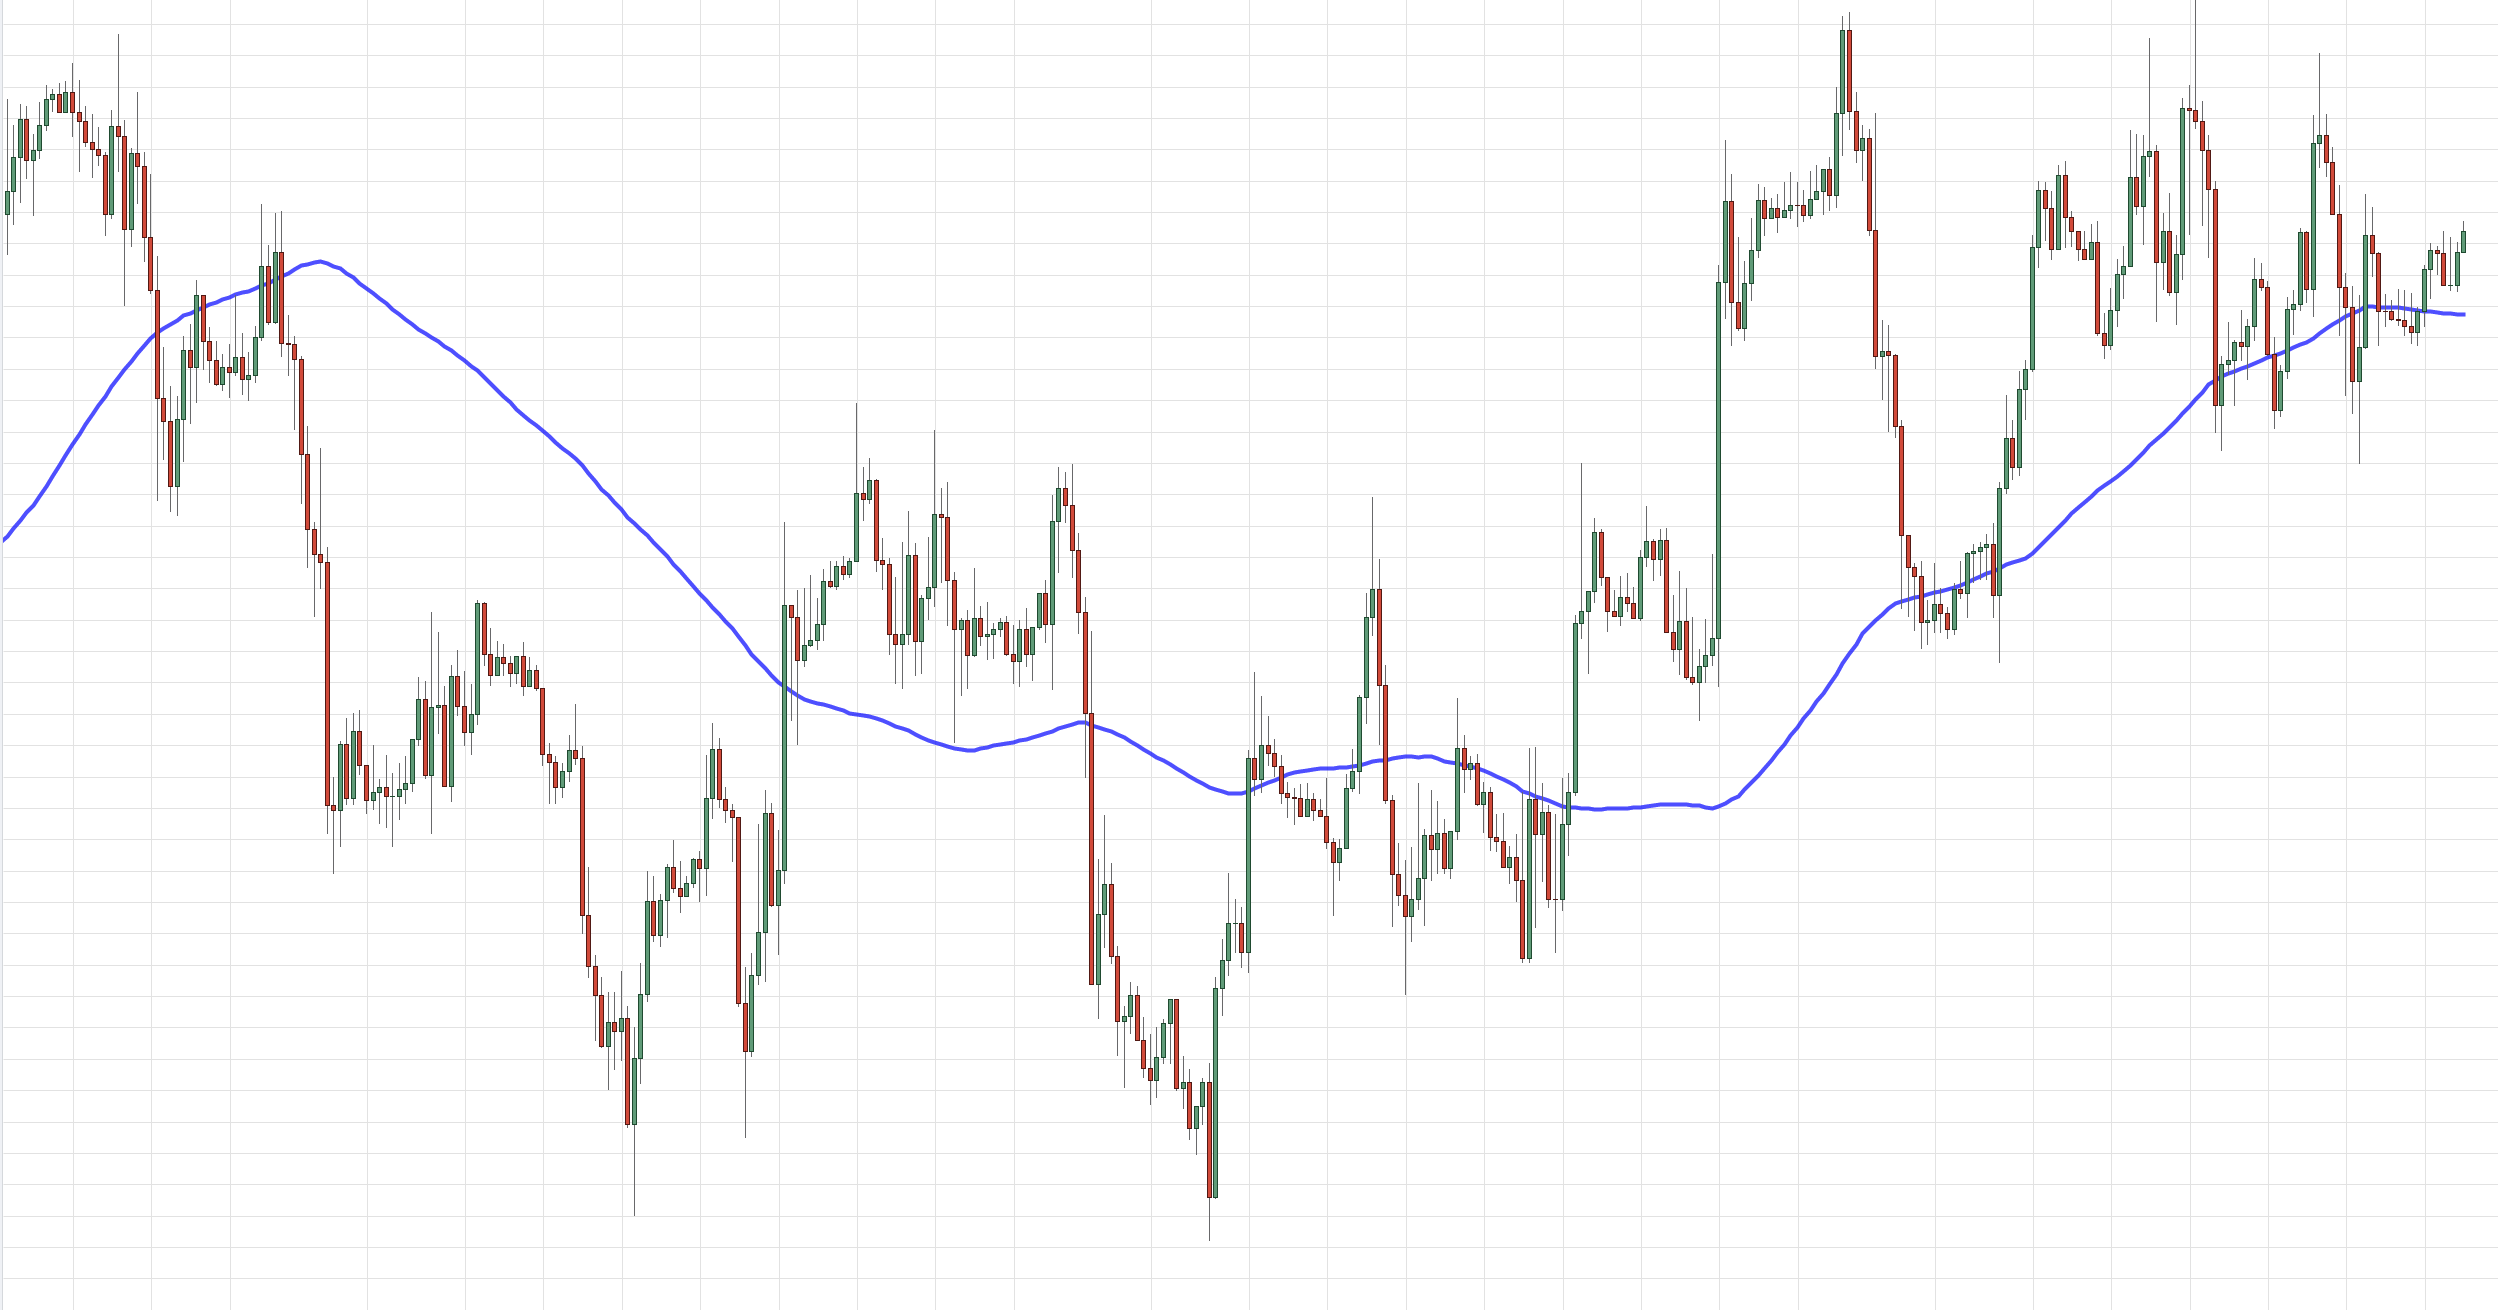
\includegraphics[width=0.8\textwidth]{img/fitting1.png}
% \label{figure:fitting1}
% \end{figure}

% \begin{figure}
% \caption{Fitting2}
% \centering
% 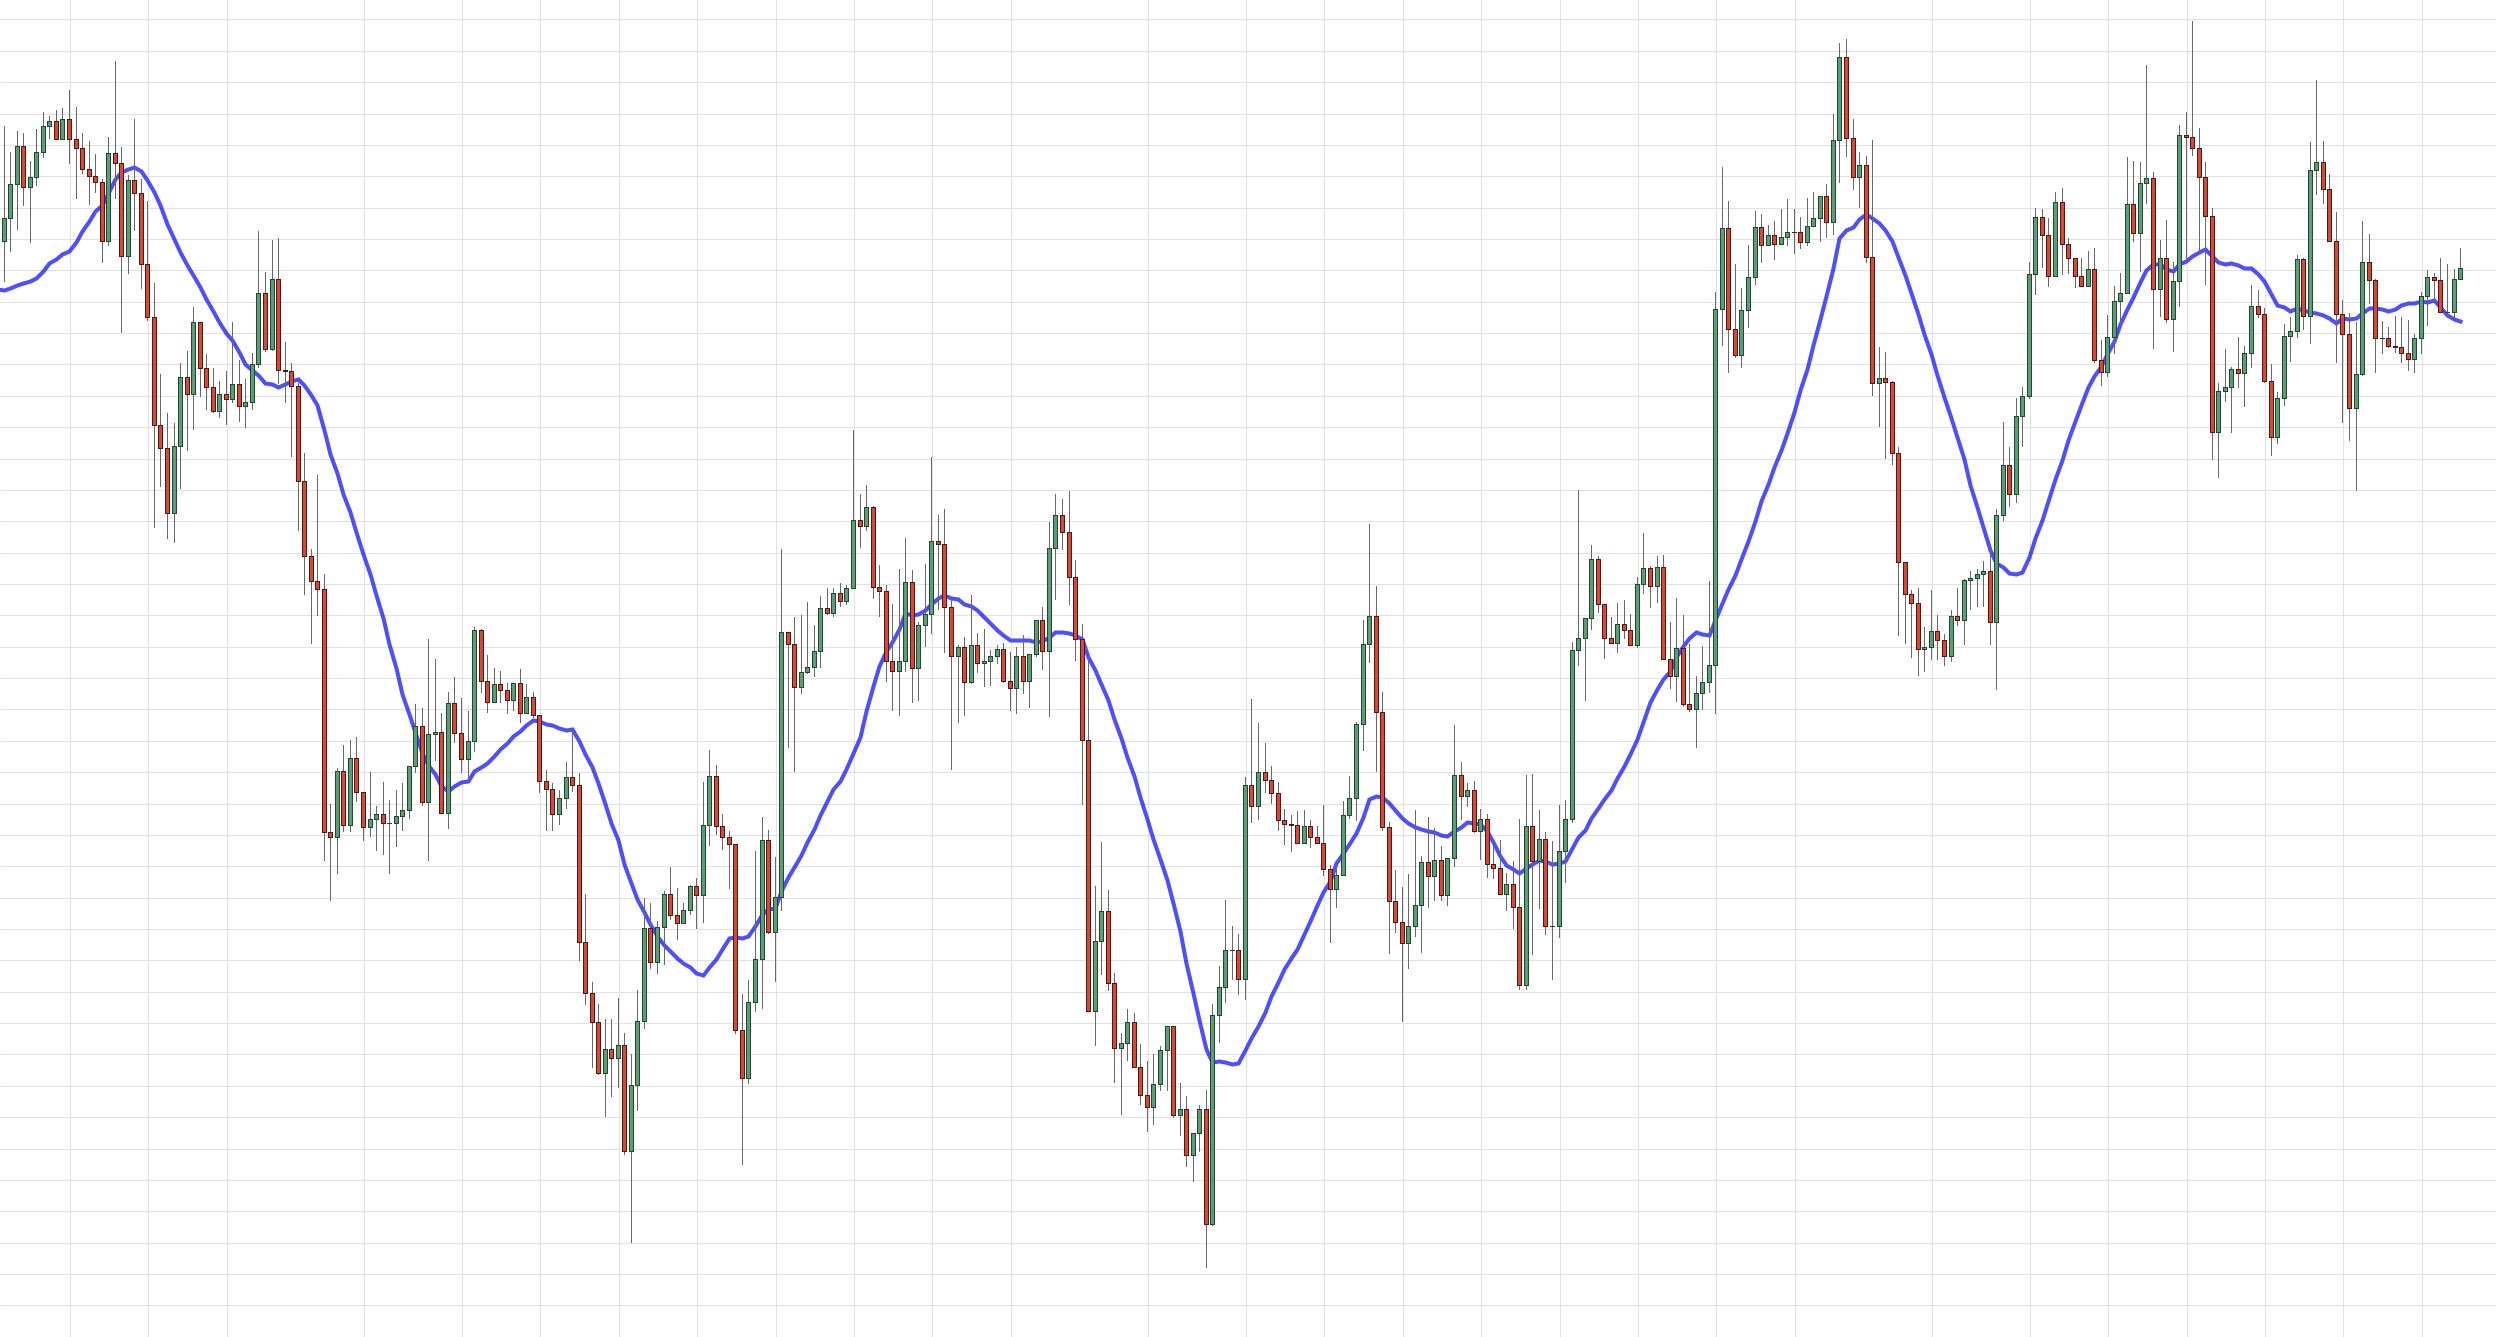
\includegraphics[width=0.8\textwidth]{img/fitting2.png}
% \label{figure:fitting2}
% \end{figure}

\section{Implementation}
\label{section:implementation}

The agents in the prediction models are represented as objects with
the following properties: agent's rules, which stores an
intuitionistic fuzzy system; activations, which stores the antecedents
of the fuzzy system; and activation thresholds, which stores the
levels that need to be surpassed by a set of inputs in order to
activate the agent.

Indeterminacy in an agent's fuzzy system is determined randomly and
optimal values are found with the metaheuristic described in
Subsection \ref{subsection:meta-heuristic}. In order to obtain
intuitionistic fuzzy sets where \ref{eq:intuitionistic-interval} holds
true, our implementation generates membership functions where the
greatest possible grade of membership is $M$ and non-membership
functions where the greatest possible grade of non-membership is $1 -
M$. The mean and spread of the Gaussian membership functions are
equal to the mean and spread of the Gaussian non-membership functions
in all cases.

The agents that are randomly generated for the meta-heuristic need to
pass a test before they can be considered a candidate to be part of a
predictive model. Considering a training data set, an agent's
activation functions are evaluated against the inputs set obtained
from that training data set in order to generate a set of activations,
where each activation is the equivalent of calculating the grade of
membership associated to a set of input. After performing this step,
all the activations are summed to obtain a score that represents the
intensity to which that agent reacts to that a set of inputs. This
score is defined by \ref{equation:activation-score}. The scores
associated to each set of inputs are ordered in a descending manner,
so the first elements are the scores that represent those sets of
inputs that would fire an agent's consequents the most. The ordered
scores list is also used to obtain the outputs that are associated to
these ordered scores, so we can know what are the outputs that the
agent \textit{should} evaluate to given those particular sets of
inputs. The resulting set of outputs are used to determine if the
agent is a suitable candidate; if most of the outputs associated to
the highest scores have the same direction (negative or positive),
then it is a suitable candidate. This mechanism ensures that the
chosen agents are specialized in similar inputs that yield similar
outputs. For our implementation, the highest scores have to be
associated to outputs that share the same direction at least 66\% of
the time.

\begin{equation}
  \label{equation:activation-score}
  A_{iCoA} = \dfrac{\sum_{i=1}^{N} i\mu_{A}(x) x_{i}}{\sum_{i=1}^{N}
    i\mu_{A}(x)}
\end{equation}

The optimization process for the predictive models loads configuration
files as its first step, depending on the market that we want to use
to obtain training and testing data sets. These configuration files
set parameters for the proposed method, such as the train-test ratio
and number of inputs, outputs and number of rules for the agents'
fuzzy systems.

For our implementation of the proposed method we chose Common Lisp as
our language, so we could use a software library for the creation of
intuitionistic fuzzy systems that we implemented in the past
\cite{Hernandez-Aguila2016} \cite{Hernandez-Aguila2017-2}. All the
populations are compressed and stored in a PostgreSQL database, which
enables us to resume the optimization of a model at any
time. Storing the populations in a database also enables us to use
populations of agents to be tested in other data sets, as well as to
extract agents from certain populations to be used in other prediction
models.

The evaluation of the agents proved to be a computationally expensive
task, as the system needs to evaluate hundreds of fuzzy systems per
iteration in the optimization process. For this reason, we implemented
a caching system where the output of an agent is stored in memory
using a technique called \textit{memoization}
\cite{johnson1995memoization} in a functional programming
context. After \textit{memoizing} an agent, if that agent is required
to be evaluated given exactly the same inputs as the ones used during
the \textit{memoization} process, then we can assume that the output
will be the same, and thus we can simply query for the output stored
in memory. The caching system prevents our implementation from
re-evaluating hundreds of fuzzy systems in the optimization process.

% I think this is a highlight, maybe going to intro  and abstract if this was
% tested - Mario
% TODO 37: COMPLETE. This was not tested, unfortunately. That's why I considered this
% only to be a technical peculiarity. Add a note if you still consider this to be
% a highlight worthy of being mentioned in the abstract and intro.

% The cahed of agents sounds interesting, maybe you should mentioned it
% if it reduced the training time - M
% TODO 38: COMPLETE. Added a paragraph explaining the caching system.

% We're using Common Lisp, an implementation of an intuitionistic fuzzy system
% We're saving our populations into a database, we can create branches, we can resume experiments.
% We're compressing our populations
% We're storing different metrics: MAPE, MASE, MAE, MSE, RMSE, Recall, Precision, F1-score, Accuracy, Revenue.
% MASE is not good if using activations because it depends on the next forecast.
% Storing popluations on a PostgreSQL database.
% Each individual agent can be evaluated to know what would be its trades given a data set.
% Agents are cached to improve computation performance.

% Activations are precomputed using if-membership. Indeterminacy is taken into account.
% Activations are reduced (summed) and we choose the greatest one (the one it is more fit to react to).
% We obtain what's the "wanted direction" (buy or sell) of that trade (the one with the greatest activation).
% Then I check the activations, ordered by how well they performed for this agent.
% The next N activations must be of the same direction than the first one. Discard agent otherwise.
% If all of them pass, then the activation threshold is the one at Nth position. So in theory each agent will trade N times, most of the time.

% Inderminacy is randomly determined from 0 to 1.
% The meta-heuristic will find heuristically if indeterminacy helps or not to activate or not.
% Already mentioned in proposed method I think: We take prices to be used as the means.

% An agent won't trade unless its inputs reach certain activation threshold.
% We check every trade to see if the agent trades or not.
% In case it passes: We use each input (price) to the fuzzy system, it fires a consequent, we do union, then if-coa, we obtain the mean of all these rules.
% Required activations (consecutive winning streak or we don't accept the agent).

% In draw optimization we're either removing an agent and checking if it's better or adding a new one and check if it's better.

% For each market we load configuration files that we determined heuristically, at random.
% We have a general file which indicates the percentage to use as test set, required activations, delta-gap, how many cores to use, what provider to use.
% Begin and end of datasets, extracts rates into global variable,
% We also have per-market config files that indicate how many data points to use as training data set, number of inputs, number of rules, inputs function.
% In experiments we provide the list of configurations per market.
% If no specific configuration file is found we use a predetermined configuration.

% We represent an agent as class that has the following slots: rules, activations, activation-threshold, consecutive-activations.

% We can use a population to be tested on any market, regardless of for what market that agent was trained for.
% List preprocessing functions:

% io-closes
% io-volumes
% io-highs
% io-lows
% io-high-heights
% io-low-heights
% io-candle-heights
% io-deltas
% io-full-heights
% io-fibos
% io-stochastic-oscillator
% io-sma
% io-awma
% io-ema
% io-macd
% io-macd-signal

\section{Experiments}
\label{section:experiments}

In order to determine the efficacy of the proposed method, we designed
experiments that involved data sets and performance metrics used in
the work by Munkhdalai et al. \cite{Munkhdalai2019}. In
\cite{Munkhdalai2019}, daily prices for the following Forex markets
are used: EUR/USD, USD/JPY, USD/CHF, GBP/USD, USD/CAD and AUD/USD. The last
year of prices are used as their data set, although they do not
provide the exact starting and ending dates. Their datasets are
partitioned into three parts: training, validation and test sets,
where the training set corresponds to 80\% of the data set, the
validation set corresponds to 10\% of the data set, and the test set
correspond to 10\% of the data set. The authors used a 5-fold time
series cross-validation method to obtain their performance metrics,
which were root-mean-squared error (RMSE) and mean-absolute error (MAE).

For our experiments, we decided to use random samples of 63 trading
days---which corresponds to a quarter of the trading days in a
year---for our data sets, which can be extracted from the last 5000
trading days (from August 28th 2004 to May 18th 2020). These data sets
are split into two parts, a training data set which corresponds to
70\% of the data set, and a test data set which corresponds to 30\% of
the data set. As a consequence, a validation step was not involved in
our experiments. Regarding the performance metrics, we provide results
using RMSE and MAE, in order to compare against the results presented
in \cite{Munkhdalai2019}, and we also provide results using mean
absolute percentage error (MAPE) and mean squared error (MSE). A total
of 30 experiments were performed for each forex market, and we provide
the means and standard deviations for each of our performance metrics
in Section \ref{section:results}.

In \cite{Munkhdalai2019}, the results of several predictive models are
provided. In order to obtain the hyper-parameters of the different
algorithms, random searching was used, with the exception of deep
learning neural networks (recurrent neural networks (RNN), long
short-term memory (LSTM) neural networks, and gated recurrent unit
(GRU) neural networks), where the learning rate was set at 0.001 using
the Adam optimizer \cite{kingma2014adam}, batch size at 64 instances
for each iteration, MSE as the loss function,and maximum number of
epochs at 3000 for the first fold, and then they used 300 epochs with
the first pre-trained model for the remaining folds. Regarding
multi-layer perceptrons (MLP), the authors used an input layer of 5 neurons
(for the prices of the last 5 days), a hidden layer of 16 neurons and
an output layer of 1 neuron (for the prediction of the next day's
price). In addition to neural network-based algorithms,
\cite{kingma2014adam} also provides results for models obtained by
random forest, AdaBoost, XGBoost and SVM
architectures.

Our MAS were optimized for 100 iterations and the loss
function was set to be RMSE. The agents in the MAS
have to trade at least 6 out of 9 (66\%; see Section
\ref{section:implementation}) trades in the same direction, regarding
their activations. We obtained the parameters shown in Table
\ref{agents-parameters} by trial and error. In Table
\ref{agents-parameters}, $HH$ means ``high height'', and represents
the price difference between the high and the greater price between
close or open prices of a trading day; $LH$ means ``low height'', and
represents the price difference between the low and the lesser price
between close or open prices of a trading day; $CH$ means ``candle
height'' and represents the absolute price difference between the open
and close prices of a trading day; and the subscript following each of
the aforementioned abbreviations represents the number of past trading
days that were considered.

% Change table and figures' captions.
% TODO 39: COMPLETE. I'll do this for TODO #47.

\begin{table}[]
  \caption{Multi-agent systems parameters}
  \small
  \centering
  \begin{tabular}{cccc}
    \textbf{Market} & \textbf{\# of Inputs} & \textbf{\# of Rules} & \textbf{Inputs} \\
    EUR/USD & 9 & 3 & $HH_3$, $LH_3$, $CH_3$ \\
    USD/JPY & 9 & 6 & $HH_3$, $LH_3$, $CH_3$ \\
    USD/CHF & 12 & 2 & $HH_4$, $LH_4$, $CH_4$ \\
    GBP/USD & 9 & 3 & $HH_3$, $LH_3$, $CH_3$ \\
    USD/CAD & 12 & 2 & $HH_4$, $LH_4$, $CH_4$ \\
    AUD/USD & 9 & 3 & $HH_3$, $LH_3$, $CH_3$ \\
  \end{tabular}
  \label{agents-parameters}
\end{table}

\section{Results}
\label{section:results}

Tables \ref{table:comparison-rmse} and \ref{table:comparison-mae} show
subsets of the results presented by Munkhdalai et
al. \cite{Munkhdalai2019}. In the case of neural networks (RNN, GRU,
LSTM and MLP), Tables \ref{table:comparison-rmse} and
\ref{table:comparison-mae} show the results obtained by Munkhdalai et
al., as well as the worst and best results that are not obtained by
using the activation function proposed by Munkhdalai et al. In
addition to the neural network-based results, results for the
predictive models based on random forest, AdaBoost, XGBoost and
SVM are also provided. The purpose of these Tables
is to provide a comparison between the predictive models generated by
our proposed method and the predictive models generated by other
methods.

Our results can be found at the bottom of the Tables, and the best
result for each market is shown in bold. Two results are presented for
our method: one where activation functions (AF) are used to restrict agents
from certain trades, and another for agents not using activation
functions to restrict their decisions. It is noteworthy that these
results cannot provide conclusive proof that one method is better than
another, as the testing datasets and methods are not the
same. Nevertheless, the reader can notice that our method is
competent, relative to the other methods presented in the Tables.

% Explain what's AF.
% TODO 40: COMPLETE.

\begin{table*}[t]
  \caption{Comparison RMSE}
  \small
  \centering
  \begin{tabular*}{0.9\textwidth}{c @{\extracolsep{\fill}} ccccccc}
    \hline
    \textbf{Model} & \textbf{Activation function} & \textbf{EUR/USD} & \textbf{USD/JPY} & \textbf{USD/CHF} & \textbf{GBP/USD} & \textbf{USD/CAD} & \textbf{AUD/USD} \\
    \hline

           & Sigmoid & 0.0079 & 6.0677 & 0.0097 & 0.0188 & 0.0075 & 0.0090 \\
    RNN    & Swish & 0.0059 & 0.6435 & 0.0062 & 0.0099 & 0.0085 & 0.0054 \\
           & Munkhdalai et al. & \textbf{0.0057} & 0.5993 & 0.0059 & 0.0098 & 0.0062 & \textbf{0.0045} \\

    \hline

           & Cosine & 0.0129 & 2.6072 & 0.0168 & 0.0548 & 0.0133 & 0.0187 \\
    GRU    & Linear & 0.0058 & 0.6054 & 0.0061 & 0.0104 & 0.0066 & 0.0052 \\
           & Munkhdalai et al. & 0.0059 & 0.6871 & 0.0060 & 0.0083 & 0.0060 & 0.0082 \\

    \hline

           & ReLU & 0.0069 & 1.6890 & 0.0079 & 0.0155 & 0.0074 & 0.0058 \\
    LSTM   & Swish & 0.0061 & 0.6890 & 0.0072 & 0.0088 & 0.0081 & 0.0069 \\
           & Munkhdalai et al. & 0.0062 & 0.6757 & 0.0087 & 0.0092 & 0.0078 & 0.0055 \\
    
    \hline

           & ReLU & 0.0064 & 0.9711 & 0.0081 & 0.0217 & 0.0066 & 0.0048 \\
    MLP    & Swish & 0.0058 & 0.9360 & 0.0061 & 0.0097 & 0.0070 & 0.0054 \\
           & Munkhdalai et al. & 0.0061 & 0.7722 & 0.0082 & 0.0088 & 0.0064 & 0.0053 \\

    \hline

    \multicolumn{2}{l}{Random forest} & 0.0068 & 0.6781 & 0.0081 & 0.0244 & 0.0075 & 0.0056 \\
    \multicolumn{2}{l}{AdaBoost} & 0.0076 & 0.8198 & 0.0136 & 0.0238 & 0.0080 & 0.0082 \\
    \multicolumn{2}{l}{XGBoost} & 0.0076 & 0.6554 & 0.0071 & 0.0241 & 0.0085 & 0.0058 \\
    \multicolumn{2}{l}{SVM} & 0.0332 & 0.6387 & 0.0394 & 0.0329 & 0.0125 & 0.0200 \\

    \hline
    \hline

    \multicolumn{2}{l}{Ours without AF}        & \textbf{0.0057}          & \textbf{0.5391}          & \textbf{0.0047}          & 0.0079          & \textbf{0.0057}          & 0.0052 \\
    \multicolumn{2}{l}{Ours with AF}           & 0.0071                   & 0.5630                   & 0.0051                   & \textbf{0.0078} & \textbf{0.0057}          & 0.0058 \\
    % \multicolumn{2}{l}{Ours with AF as weight} & \textbf{0.0052} & \textbf{0.4625} & \textbf{0.0042} & 0.0084          & \textbf{0.0047} & \textbf{0.0050} \\

    \hline

  \end{tabular*}
  \label{table:comparison-rmse}
\end{table*}

\begin{table*}[t]
  \caption{Comparison MAE}
  \small
  \centering
  \begin{tabular*}{0.9\textwidth}{c @{\extracolsep{\fill}} ccccccc}
    \hline
    \textbf{Model} & \textbf{Activation function} & \textbf{EUR/USD} & \textbf{USD/JPY} & \textbf{USD/CHF} & \textbf{GBP/USD} & \textbf{USD/CAD} & \textbf{AUD/USD} \\
    \hline

          & Sigmoid & 0.0060 & 5.4000 & 0.0081 & 0.0126 & 0.0060 & 0.0079 \\
    RNN   & Swish & 0.0044 & 0.4925 & 0.0042 & 0.0074 & 0.0068 & 0.0043 \\
          & Munkhdalai et al. & 0.0043 & 0.4479 & 0.0037 & 0.0083 & 0.0047 & 0.0034 \\
    \hline
          & Cosine & 0.0098 & 2.0191 & 0.0130 & 0.0396 & 0.0106 & 0.0162 \\
    GRU   & Linear & 0.0044 & 0.4475 & 0.0041 & 0.0083 & 0.0052 & 0.0041 \\
          & Munkhdalai et al. & 0.0044 & 0.5327 & 0.0039 & 0.0062 & 0.0046 & 0.0071 \\
    \hline
          & ReLU & 0.0053 & 1.4920 & 0.0054 & 0.0101 & 0.0058 & 0.0046 \\
    LSTM  & Swish & 0.0045 & 0.5243 & 0.0049 & 0.0065 & 0.0063 & 0.0054 \\
          & Munkhdalai et al. & 0.0046 & 0.5200 & 0.0060 & 0.0069 & 0.0061 & 0.0044 \\
    \hline

          & ReLU & 0.0049 & 0.7499 & 0.0058 & 0.0150 & 0.0052 & 0.0038 \\
    MLP   & Swish & 0.0043 & 0.7351 & 0.0039 & 0.0073 & 0.0055 & 0.0042 \\
          & Munkhdalai et al. & 0.0047 & 0.6114 & 0.0059 & 0.0066 & 0.0049 & 0.0041 \\
          

    \hline

    \multicolumn{2}{l}{Random forest} & 0.0053 & 0.5209 & 0.0061 & 0.0156 & 0.0059 & 0.0044 \\
    \multicolumn{2}{l}{AdaBoost} & 0.0059 & 0.6440 & 0.0103 & 0.0158 & 0.0063 & 0.0066 \\
    \multicolumn{2}{l}{XGBoost} & 0.0059 & 0.4958 & 0.0048 & 0.0156 & 0.0064 & 0.0045 \\
    \multicolumn{2}{l}{SVM} & 0.0304 & 0.4718 & 0.0376 & 0.0294 & 0.0099 & 0.0176 \\

    \hline
    \hline
    
    \multicolumn{2}{l}{Ours without AF}        & 0.0050          & 0.4903          & 0.0041          & 0.0073          & 0.0050          & 0.0048 \\
    \multicolumn{2}{l}{Ours with AF}           & \textbf{0.0033} & \textbf{0.1810} & \textbf{0.0019} & \textbf{0.0038} & \textbf{0.0033} & \textbf{0.0027} \\
    % \multicolumn{2}{l}{Ours with AF as weight} & 0.0044          & 0.4122          & 0.0036          & 0.0069          & 0.0042          & 0.0044 \\

    \hline

  \end{tabular*}
  \label{table:comparison-mae}
\end{table*}

% Tables \ref{table:full-results-no-activations}
% \ref{table:full-results-activations}
% and \label{table:full-results-weights} provide results involving
% different versions of our proposed method. Table
% \ref{table:full-results-no-activations} shows results for a
% multi-agent system where agents have no activation functions---which
% means that agents respond to any set of inputs. Table
% \ref{table:full-results-activations} shows results for a
% multi-agent system where agents have activation functions, exactly as
% described in Section \ref{section:proposed-method}. Lastly, Table
% \ref{table:full-results-activations} shows results for a modified
% version of our proposed method, where the output of an agent's
% activation function is used a weight that is multipiled by that
% agent's output, instead of using the activation function as a
% threshold, as in the proposed method.

Tables \ref{table:full-results-no-activations}
and \ref{table:full-results-activations} provide results involving
different versions of our proposed method. Table
\ref{table:full-results-no-activations} shows results for a
MAS where agents have no activation functions---which
means that agents respond to any set of inputs. Table
\ref{table:full-results-activations} shows results for a
MAS where agents have activation functions, exactly as
described in Section \ref{section:proposed-method}.

\begin{table*}[t]
  \caption{Multi-agent system without activation functions}
  \small
  \centering
  \begin{tabular*}{0.9\textwidth}{c @{\extracolsep{\fill}} ccccccc}
    \hline
    \multicolumn{2}{c}{\textbf{Metric}} & \textbf{EUR/USD} & \textbf{USD/JPY} & \textbf{USD/CHF} & \textbf{GBP/USD} & \textbf{USD/CAD} & \textbf{AUD/USD} \\
    \hline
    \multirow{2}{*}{MAE} & Mean & 5.03\e{-03} & 4.90\e{-01} & 4.13\e{-03} & 7.34\e{-03} & 5.05\e{-03} & 4.83\e{-03} \\
                      & Std dev & 2.79\e{-03} & 2.20\e{-01} & 1.94\e{-03} & 4.01\e{-03} & 2.24\e{-03} & 2.12\e{-03} \\
    \hline
    \multirow{2}{*}{MAPE} & Mean & 4.49\e{-03} & 2.89\e{-01} & 3.70\e{-03} & 6.53\e{-03} & 4.51\e{-03} & 4.32\e{-03} \\
                       & Std dev & 2.47\e{-03} & 1.01\e{-01} & 1.73\e{-03} & 3.50\e{-03} & 1.99\e{-03} & 1.88\e{-03} \\
    \hline
    \multirow{2}{*}{MSE} & Mean & 4.20\e{-05} & 3.52\e{-01} & 2.76\e{-05} & 9.21\e{-05} & 3.92\e{-05} & 3.35\e{-05} \\
                      & Std dev & 5.01\e{-05} & 3.37\e{-01} & 2.98\e{-05} & 1.36\e{-05} & 4.06\e{-03} & 3.12\e{-05} \\
    \hline
    \multirow{2}{*}{RMSE} & Mean & 5.69\e{-03} & 5.39\e{-01} & 4.69\e{-03} & 7.93\e{-03} & 5.70\e{-03} & 5.18\e{-03} \\
                       & Std dev & 3.18\e{-03} & 2.51\e{-01} & 2.09\e{-03} & 4.83\e{-03} & 2.64\e{-03} & 2.34\e{-03} \\
    
    \hline
  \end{tabular*}
  \label{table:full-results-no-activations}
\end{table*}

\begin{table*}[t]
  \caption{Multi-agent system with binary activation functions}
  \small
  \centering
  \begin{tabular*}{0.9\textwidth}{c @{\extracolsep{\fill}} ccccccc}
    \hline
    \multicolumn{2}{c}{\textbf{Metric}} & \textbf{EUR/USD} & \textbf{USD/JPY} & \textbf{USD/CHF} & \textbf{GBP/USD} & \textbf{USD/CAD} & \textbf{AUD/USD} \\
    \hline
    \multirow{2}{*}{MAE} & Mean & 3.27\e{-03} & 1.81\e{-01} & 1.95\e{-03} & 3.80\e{-03} & 3.32\e{-03} & 2.74\e{-03} \\
                      & Std dev & 3.81\e{-03} & 1.31\e{-01} & 1.53\e{-03} & 3.12\e{-03} & 1.94\e{-03} & 2.25\e{-03} \\
    \hline
    \multirow{2}{*}{MAPE} & Mean & 6.04\e{-03} & 2.93\e{-01} & 3.92\e{-03} & 6.10\e{-03} & 4.53\e{-03} & 5.53\e{-03} \\
                       & Std dev & 4.38\e{-03} & 1.50\e{-01} & 2.47\e{-03} & 3.19\e{-03} & 2.07\e{-03} & 3.20\e{-03} \\
    \hline
    \multirow{2}{*}{MSE} & Mean & 6.81\e{-05} & 2.62\e{-01} & 2.95\e{-05} & 6.46\e{-05} & 3.62\e{-05} & 5.25\e{-05} \\
                      & Std dev & 9.54\e{-05} & 2.52\e{-01} & 3.55\e{-05} & 6.77\e{-05} & 3.29\e{-05} & 5.49\e{-05} \\
    \hline
    \multirow{2}{*}{RMSE} & Mean & 7.12\e{-03} & 5.63\e{-01} & 5.11\e{-03} & 7.79\e{-03} & 5.70\e{-03} & 5.81\e{-03} \\
                       & Std dev & 5.15\e{-03} & 2.98\e{-01} & 3.21\e{-03} & 4.05\e{-03} & 2.36\e{-03} & 3.72\e{-03} \\

    \hline
  \end{tabular*}
  \label{table:full-results-activations}
\end{table*}

% \begin{table*}[t]
%   \caption{Multi-agent system with activation functions as weights}
%   \small
%   \centering
%   \begin{tabular*}{0.9\textwidth}{c @{\extracolsep{\fill}} ccccccc}
%     \hline
%     \multicolumn{2}{c}{\textbf{Metric}} & \textbf{EUR/USD} & \textbf{USD/JPY} & \textbf{USD/CHF} & \textbf{GBP/USD} & \textbf{USD/CAD} & \textbf{AUD/USD} \\
%     \hline
%     \multirow{2}{*}{MAE} & Mean & 4.42\e{-03} & 4.12\e{-01} & 3.64\e{-03} & 6.94\e{-03} & 4.17\e{-03} & 4.40\e{-03} \\
%                       & Std dev & 1.93\e{-03} & 2.17\e{-01} & 1.58\e{-03} & 4.10\e{-03} & 1.59\e{-03} & 2.37\e{-03} \\
%     \hline
%     \multirow{2}{*}{MAPE} & Mean & 3.95\e{-03} & 2.35\e{-01} & 3.25\e{-03} & 6.15\e{-03} & 3.73\e{-03} & 3.94\e{-03} \\
%                        & Std dev & 1.71\e{-03} & 8.11\e{-02} & 1.40\e{-03} & 3.49\e{-03} & 1.41\e{-03} & 2.10\e{-03} \\
%     \hline
%     \multirow{2}{*}{MSE} & Mean & 3.31\e{-05} & 2.74\e{-01} & 2.11\e{-05} & 1.06\e{-04} & 2.63\e{-05} & 3.15\e{-05} \\
%                       & Std dev & 3.23\e{-05} & 3.33\e{-01} & 2.05\e{-05} & 2.65\e{-04} & 1.95\e{-05} & 3.69\e{-05} \\
%     \hline
%     \multirow{2}{*}{RMSE} & Mean & 5.17\e{-03} & 4.63\e{-01} & 4.18\e{-03} & 8.43\e{-03} & 4.68\e{-03} & 4.99\e{-03} \\
%                        & Std dev & 2.43\e{-03} & 2.36\e{-01} & 2.00\e{-03} & 6.53\e{-03} & 1.85\e{-03} & 2.67\e{-03} \\

%     \hline
%   \end{tabular*}
%   \label{table:full-results-weights}
% \end{table*}

\section{Conclusion}
\label{section:conclusion}

% Check that we mention all of these contributions in here:
% i) our method describes a novel architecture that mixes MAS and fuzzy systems for
% the creation of predictive models;
% x ii) the activation functions found in the agents' fuzzy systems help to decrease the error between
% predicted and real market prices;
% iii) the results from the experiments indicate us that the models generated by our method are
% competitive against models generated by deep learning, random forest,
% AdaBoost, XGBoost and support-vector machines;
% iv) our method describes a simple and effective method for the tuning of parameters for MAS.
% TODO 41: COMPLETE.

Our method creates an architecture that successfully mixes MAS and
fuzzy systems for the creation of predictive models. The generated
predictive models are optimized by a simple but effective
meta-heuristic, which is able to find satisfactory solutions in a
relatively low number of iterations (100, in the case of the
experiments presented in this work).

After examining Tables \ref{table:comparison-rmse} and
\ref{table:comparison-mae}, we can conclude that our method proves to
be competitive for predicting the six forex markets EUR/USD, USD/JPY,
USD/CHF, GBP/USD, USD/CAD and AUD/USD, after being compared against
models generated by RNN, LSTM, GRU, MLP, random forest, AdaBoost,
XGBoost and SVM.

In the case of Table \ref{table:comparison-rmse}---which
considers RMSE as the loss function---, we can see that our method
performed the best without using activation functions in the agents'
fuzzy systems, with the exception of GBP/USD. For EUR/USD, the method
presented in \cite{Munkhdalai2019} performed as well as our method,
and outperformed ours for AUD/USD. On the other hand, Table
\ref{table:comparison-mae}---which considers MAE as the loss
function---shows that our method performed the best for every forex
market.

RMSE has been critized before \cite{willmott2005advantages}
\cite{willmott2009ambiguities} as being an ambiguous measure of
average error, where MAE is not, but it has also been reported to be
more suitable than MAE when the error distribution is expected to be
Gaussian \cite{chai2014root}, which is the case for the presented
work. If we consider RMSE to be a more suitable metric to measure the
performance of our models, we can conclude that our method performs
better in most of the markets without the use of activation functions
in the agents' fuzzy systems. Nevertheless, the use of activation
functions restricts the predictive models to trade in some cases,
which would yield a non-Gaussian error distribution. Considering this
restriction, it may be more prudent to consider MAE as a better metric
to measure the performance of our method with activation functions
against our method without activation functions, and we could conclude
that the use of activation functions dramatically improves our
method's performance.

% Say this in the abstract - Mario
% TODO 42: COMPLETE. I'm not adding it because the abstract word limit is almost reached.

Finally, it must be noted that the results depicted in
\ref{table:comparison-rmse} and \ref{table:comparison-mae} have the
purpose of demonstrating the competitiveness of our method for the
creation of predictive models. Concluding that our method is better
than the others shown in those tables would be naive, as the datasets
used in our experiments and the methods used for testing the
performance of the models differ to those used in
\cite{Munkhdalai2019}.

\section{Future Work}
\label{section:future-work}

The experiments presented in this work demonstrate that better
methodologies need to be used in order to provide conclusive proof
that the use of activation functions in the agents' fuzzy systems is
beneficial for the creation of predictive models. Additionally, we can
test our activation functions in other methods, such as neural
networks. Furthermore, we could design experiments that demonstrate
which version of our method helps real traders take better decisions.

The proposed method was tested using a subset of all the forex markets
currently available. More experiments could be performed where
additional forex markets are tested. Moreover, our method should be
tested with financial markets of different natures, such as stocks,
bonds, commodities and metals.

An advantage of fuzzy systems over other modelling techniques is that
fuzzy systems are interpretable. Natural language processing
techniques that use the fuzzy systems as inputs could be used to
provide texts that describe the conditions of a market, as perceived
by the agents in the MAS.

Our implementation should be adapted to perform in a distributed
manner, where agents are evaluated in parallel in different CPU cores
or even different physical machines. A distributed architecture will
help achieve results faster, which will allow us to test different
approaches for the creation of predictive models using our method.

Finally, the meta-heuristic used in the proposed method should be
tested in performance against other meta-heuristics, such as genetic
algorithms or particle swarm optimization. Finding better optimization
algorithms for our method can help us achieve results faster. It is
also probable that lower errors could be achieved, as we do not know
if our current optimization method is considering an appropriate
search space.

% We could implement a distributed algorithm
% I must add it now because I mention it in the introduction.
% Mention use other optimization algorithms.
% TODO 43: COMPLETE.

% Check when are abbreviations created and then use only the abbreviation (e.g. MAS)
% TODO 44: COMPLETE.

% Check passive voice.
% TODO 45: COMPLETE. I think, at least.

% Check formulas.
% TODO 46:

% Check captions.
% TODO 47:

% Check figures.
% TODO 48:

% Check algorithms.
% TODO 49:

% Add using our activation functions for neural networks in future work.
% TODO 50: COMPLETE.

\section*{Acknowledgment}

\begin{IEEEbiography}[{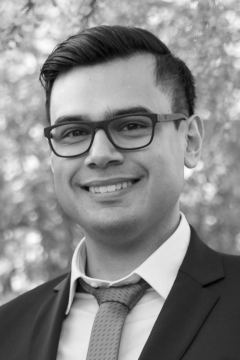
\includegraphics[width=1in,height=1.25in,clip,keepaspectratio]{img/amaury-1by1half-in.png}}]{Amaury
  Hernandez-Aguila} 
\end{IEEEbiography}

\bibliography{bibliography}
\bibliographystyle{IEEEtran}

\EOD

\end{document}
